% ============================================
% SECTION 3: Results
% ============================================
\section{Resultados}

\begin{frame}{LA-CDIP Dataset - Estatísticas}
\begin{columns}
\column{0.5\textwidth}
\textbf{Composição:}
\begin{itemize}
    \item 4.993 documentos
    \item 144 classes diferentes
    \item Min: 2 documentos/classe
    \item Max: 497 documentos/classe
    \item Mediana: 13 documentos/classe
\end{itemize}

\textbf{Splits:}
\begin{itemize}
    \item ZSL: separação completa treino/teste
    \item GZSL: 50\% overlap de classes
    \item 5-fold cross-validation
\end{itemize}

\column{0.5\textwidth}
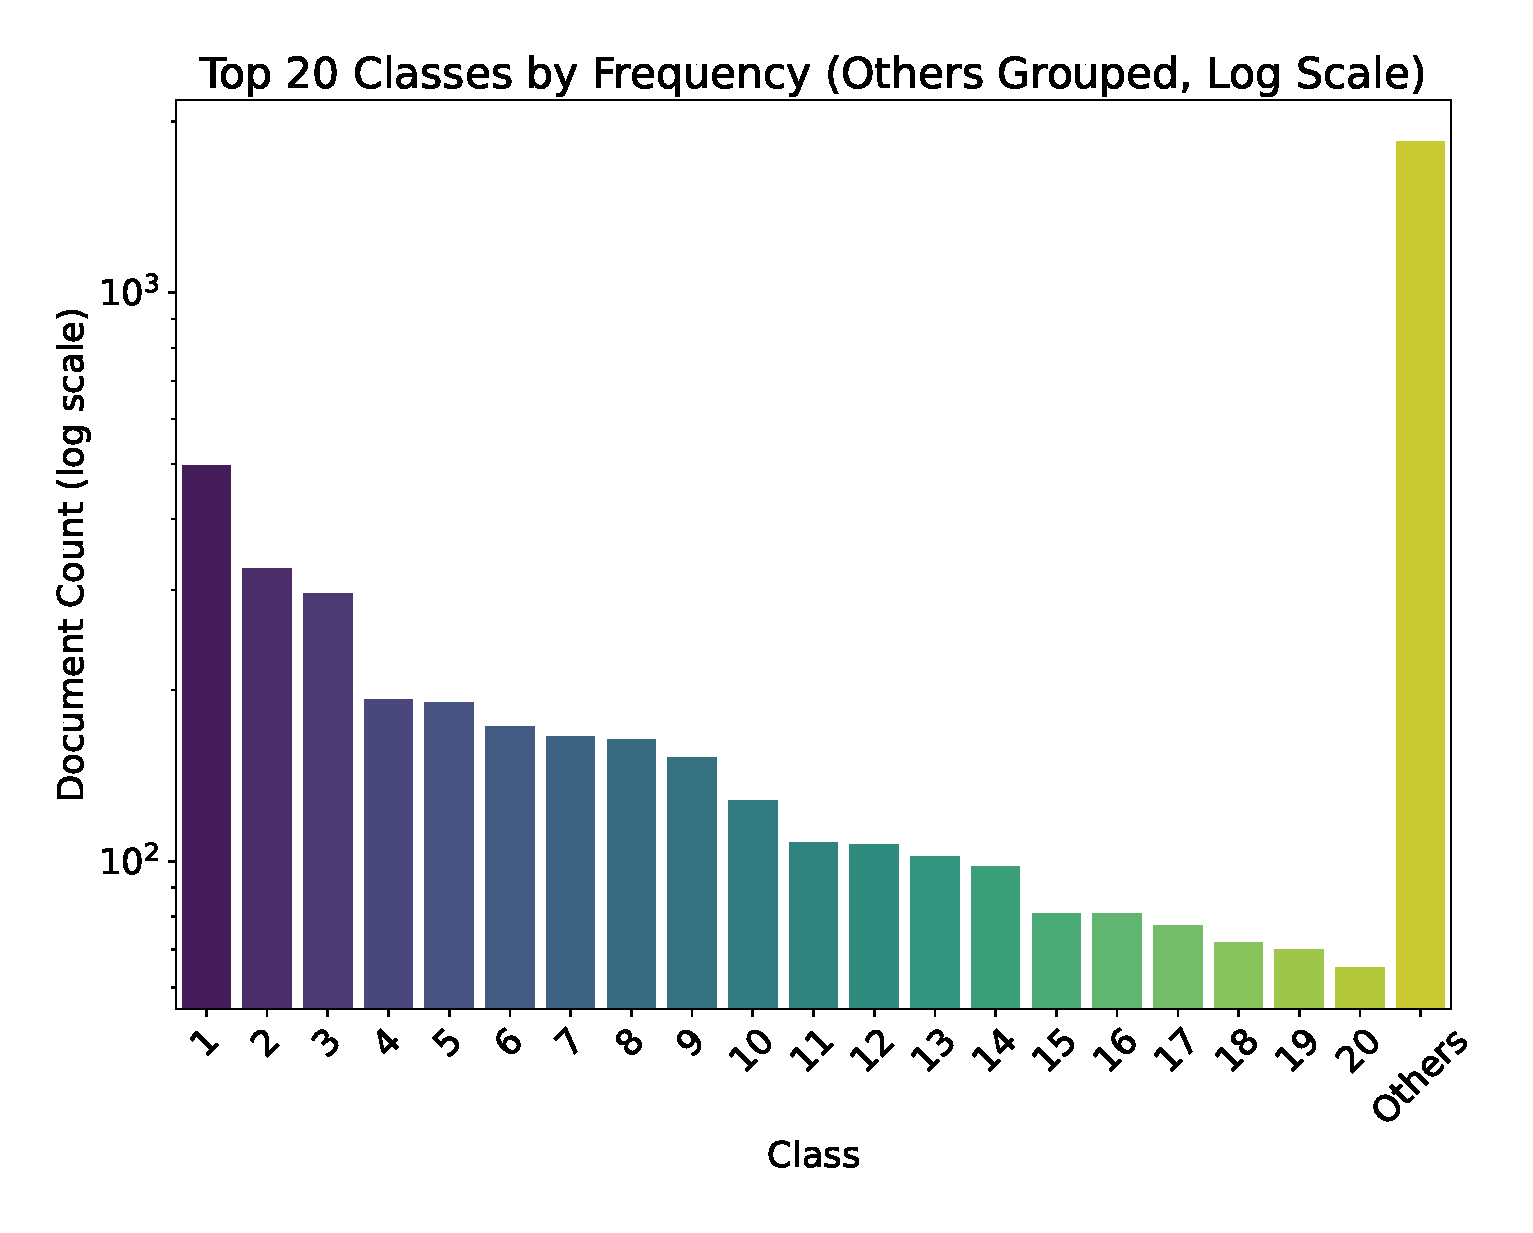
\includegraphics[width=\textwidth]{images/hist2.eps}
\end{columns}
\end{frame}

\begin{frame}{Métricas de Avaliação}
\begin{block}{Equal Error Rate (EER)}
\begin{itemize}
    \item Ponto onde FAR = FRR
    \item FAR: False Acceptance Rate
    \item FRR: False Rejection Rate
\end{itemize}
\end{block}

\begin{columns}
\column{0.5\textwidth}
\begin{equation*}
FAR(\tau) = \frac{\text{False Acceptances}}{\text{Total Negatives}}
\end{equation*}

\column{0.5\textwidth}
\begin{equation*}
FRR(\tau) = \frac{\text{False Rejections}}{\text{Total Positives}}
\end{equation*}
\end{columns}

\vspace{0.3cm}
\begin{center}
\textbf{Protocolo de Teste:}\\
Para cada documento: 1 par similar + 1 par dissimilar
\end{center}
\end{frame}

\begin{frame}{Resultados - Visão Geral}
\begin{table}
\tiny
\begin{tabular}{lclcccc}
\toprule
\textbf{Architecture} & \textbf{Edition} & \textbf{Params} & \textbf{ZSL CV} & \textbf{GZSL CV} & \textbf{Test ZSL} & \textbf{Test GZSL} \\
\midrule
ResNet & 18 & 11M & 5.03 & 1.54 & 4.98 & 1.51 \\
ResNet & 34 & 21M & 4.32 & 2.10 & 4.13 & 1.53 \\
EfficientNet & 0 & 4M & 4.41 & 2.27 & 6.02 & 0.95 \\
EfficientNet & 1 & 6M & 3.93 & 3.54 & 8.88 & 2.70 \\
VGG & 13 & 129M & 7.03 & 4.79 & 9.30 & 3.95 \\
ViT & Base & 87M & 12.43 & 7.97 & 19.72 & 5.19 \\
\midrule
GPT-4o & 2024-11-20 & * & -- & -- & 2.75 & 1.33 \\
GPT-4o mini & 2024-07-18 & * & -- & -- & 4.70 & 4.07 \\
Qwen-VL & 2.5 & 7B & -- & -- & 6.61 & 4.20 \\
InternVL & 2.5 & 8B & -- & -- & 8.58 & 10.40 \\
LLaMA & 3.2 & 11B & -- & -- & 13.95 & 21.90 \\
\bottomrule
\end{tabular}
\caption*{Mean EER (\%) - Valores menores são melhores}
\end{table}
\end{frame}

\begin{frame}{Resultados - Modelos Visuais}
\begin{block}{Principais Observações}
\begin{itemize}
    \item \textbf{Arquiteturas menores superaram as maiores}
    \begin{itemize}
        \item ResNet-18 e ResNet-34: melhor desempenho
        \item ResNet-50, 101, 152: desempenho progressivamente pior
    \end{itemize}
    
    \item \textbf{Vision Transformer (ViT): pior desempenho}
    \begin{itemize}
        \item Overfitting nos dados de treino
        \item 0\% de erro de treino, alto erro de validação
        \item Causa provável: dataset pequeno (4.993 documentos)
    \end{itemize}
    
    \item \textbf{Melhores modelos:}
    \begin{itemize}
        \item ResNet-34, EfficientNet-0 e EfficientNet-1
        \item Balanço entre tamanho e generalização
    \end{itemize}
\end{itemize}
\end{block}
\end{frame}

\begin{frame}{Resultados - Comparação ZSL vs GZSL}
\begin{columns}
\column{0.5\textwidth}
\textbf{GZSL consistentemente melhor:}
\begin{itemize}
    \item 50\% das classes vistas no treino
    \item Maior diferença em modelos grandes
    \item Overfitting mitigado no cenário mais fácil
\end{itemize}

\textbf{Test split ZSL mais desafiador:}
\begin{itemize}
    \item Alta variância entre splits
    \item Padrões completamente diferentes
    \item Taxas de erro mais altas
\end{itemize}

\column{0.5\textwidth}
\textbf{Exemplo ResNet-18:}
\begin{itemize}
    \item ZSL CV: 5.03\%
    \item GZSL CV: 1.54\%
    \item Test ZSL: 4.98\%
    \item Test GZSL: 1.51\%
\end{itemize}

\vspace{0.5cm}
\textbf{Exemplo ViT-Base:}
\begin{itemize}
    \item ZSL CV: 12.43\%
    \item GZSL CV: 7.97\%
    \item Test ZSL: 19.72\%
    \item Test GZSL: 5.19\%
\end{itemize}
\end{columns}
\end{frame}

\begin{frame}{Resultados - Large Language Models}
\begin{block}{Observações}
\begin{itemize}
    \item \textbf{GPT-4o: melhor desempenho geral}
    \begin{itemize}
        \item ZSL: 2.75\% | GZSL: 1.33\%
        \item Porém: centenas de vezes mais caro por inferência
    \end{itemize}
    
    \item \textbf{Alternativas open-source promissoras:}
    \begin{itemize}
        \item Qwen-VL 7B: desempenho próximo ao GPT-4o mini
        \item InternVL 2.5: competitivo
    \end{itemize}
    
    \item \textbf{LLaMA 3.2 Vision:}
    \begin{itemize}
        \item Limitações no manuseio de múltiplas imagens
        \item Necessário combinar imagens em input único
    \end{itemize}
    
    \item \textbf{Tendências diferentes entre cenários:}
    \begin{itemize}
        \item InternVL melhor no ZSL
        \item GPT melhor no GZSL
    \end{itemize}
\end{itemize}
\end{block}
\end{frame}

\begin{frame}{Comparação: Visual Models vs LLMs}
\begin{center}
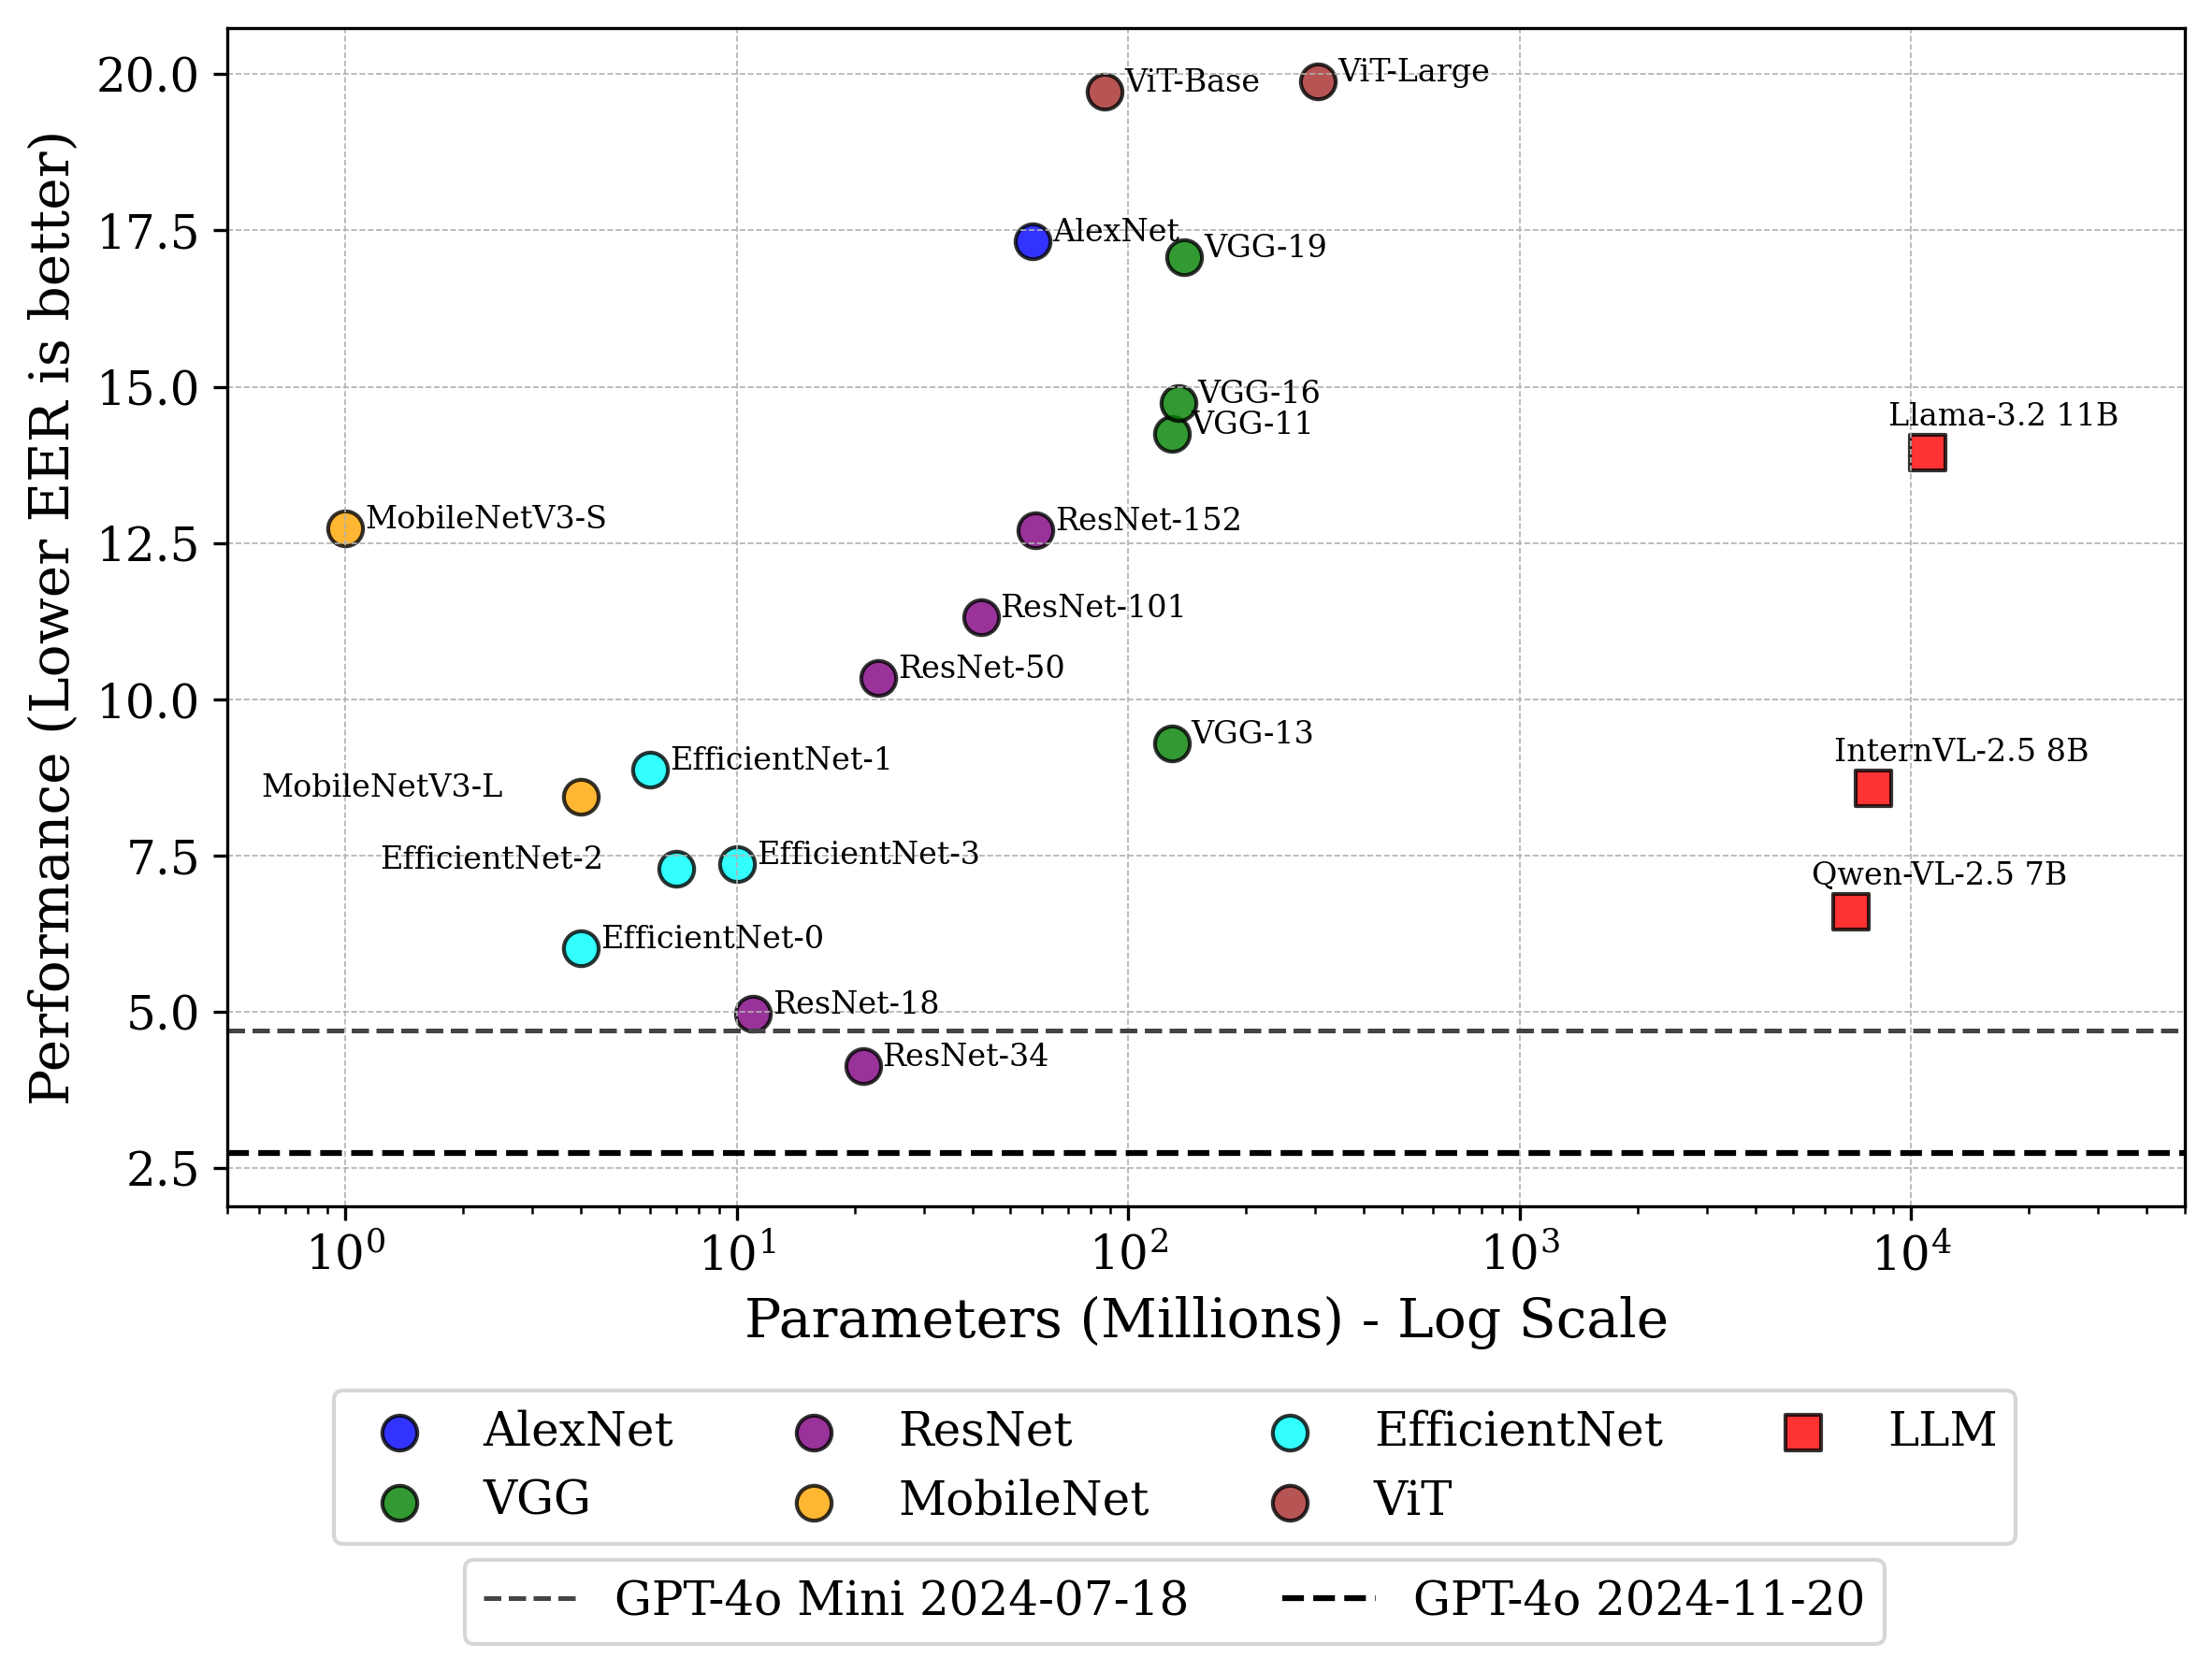
\includegraphics[width=0.85\textwidth]{images/performance_vs_parameters.png}
\end{center}

\textbf{Trade-off entre complexidade e efetividade:}
\begin{itemize}
    \item Modelos visuais leves (ResNet-18, EfficientNet-0): competitivos com muito menos parâmetros
    \item GPT-4o: ligeiro ganho de performance, mas custo muito maior
\end{itemize}
\end{frame}

\begin{frame}{Usos Industriais}
\begin{block}{Sistema de Verificação (Classificação Binária)}
\begin{itemize}
    \item Dado: documento de referência + threshold
    \item Decisão: aceitar se distância < threshold, rejeitar caso contrário
\end{itemize}
\end{block}

\begin{block}{Sistema de Identificação (Classificação Multi-classe)}
\begin{itemize}
    \item Dado: referências para cada classe + threshold
    \item Decisão: atribuir à classe mais próxima ou rejeitar se fora do threshold
\end{itemize}
\end{block}

\textbf{Design Choices:}
\begin{itemize}
    \item Múltiplas referências por classe (usar centroid)
    \item Thresholds diferentes por classe
    \item Armazenar embeddings ao invés de imagens
    \item Complexidade: O(r) verificação, O(rc) identificação
\end{itemize}
\end{frame}
